\chapter[Gaussian processes and kernels]{Gaussian processes, kernels and radial basis functions}
\label{ch:gp}

Chapter~\ref{ch:toolkit} ended with Bayesian linear regression and noticed that its predictions depend on the
features only through inner products $k(x,x') = \tau^2\phi(x)\T\phi(x')$. This chapter takes that seriously: choose
$k$ directly, let the feature space be infinite-dimensional, and the result is a Gaussian process (GP). We then show
that kriging, kernel ridge regression and radial-basis-function interpolation are the same object seen from three
disciplines, derive what a GP's error bars really mean, and explain the failure modes the study measured.

\section{From finitely many features to a Gaussian process}

\begin{definition}[Gaussian process]
A Gaussian process is a random function $f$ such that, for any finite set of points $x_1,\dots,x_n$, the vector
$\big(f(x_1),\dots,f(x_n)\big)$ is jointly Gaussian. It is fixed by a mean function $m(x) = \E[f(x)]$ and a
covariance function (\emph{kernel}) $k(x,x') = \Cov\big(f(x), f(x')\big)$. We write $f \sim \mathcal{GP}(m, k)$.
\end{definition}

Think of a GP as an infinitely long Gaussian vector indexed by $x$ instead of by an integer. You never handle the
infinite object: every computation touches only the finitely many points you have, and the marginal rule of
Chapter~\ref{ch:toolkit} (``delete the rows and columns you do not need'') guarantees that answers do not depend on
points you did not ask about.

\begin{connection}[Mercer and Karhunen--Lo\`eve: a GP is POD of a random field]
A valid kernel can be expanded as $k(x,x') = \sum_{j} \lambda_j\, \psi_j(x)\,\psi_j(x')$, where $\psi_j$ are the
eigenfunctions of the integral operator $(\mathcal{K}g)(x) = \int k(x,x')g(x')\,dx'$ and $\lambda_j \ge 0$ its
eigenvalues (\emph{Mercer's theorem}, the continuous version of the spectral theorem for the symmetric matrix $K$).
Then a GP sample can be written
\begin{equation}
  f(x) = \sum_j \sqrt{\lambda_j}\; \xi_j\, \psi_j(x), \qquad \xi_j \sim \N(0,1) \text{ independent}
  \label{eq:kl}
\end{equation}
(the \emph{Karhunen--Lo\`eve expansion}). This is exactly POD applied to a random field instead of a snapshot
matrix: $\psi_j$ are the modes, $\lambda_j$ the energies, and the decay of $\lambda_j$ says how many modes matter.
It is also Bayesian linear regression with features $\sqrt{\lambda_j}\psi_j$ and infinitely many of them. A GP is
the limit of Chapter~\ref{ch:toolkit}'s model in which you stop truncating.
\end{connection}

\section{Kernels: what they encode}

\paragraph{What makes a kernel valid.} Any covariance matrix must be PSD, so a function $k$ can be a kernel only if
every matrix $K_{ij} = k(x_i,x_j)$ is PSD, for every choice of points. Sums, products and positive multiples of
valid kernels are valid (a sum of covariances is the covariance of a sum of independent processes; a product is the
covariance of a product of independent processes), which is how kernels are built.

\paragraph{Stationary kernels.} Most surrogate work uses kernels that depend only on the separation $r =
\norm{x - x'}/\ell$, with a \emph{length-scale} $\ell$ and a signal variance $\sigma_f^2$:
\begin{align}
  \text{squared exponential (SE):}\quad & k(r) = \sigma_f^2 \exp(-r^2/2), \\
  \text{Mat\'ern } \nu = \tfrac12:\quad & k(r) = \sigma_f^2\, e^{-r}, \\
  \text{Mat\'ern } \nu = \tfrac32:\quad & k(r) = \sigma_f^2 (1 + \sqrt3\, r)\, e^{-\sqrt3 r}, \\
  \text{Mat\'ern } \nu = \tfrac52:\quad & k(r) = \sigma_f^2 \big(1 + \sqrt5\, r + \tfrac53 r^2\big) e^{-\sqrt5 r}.
\end{align}
The length-scale is the distance over which $f$ ``forgets'' its value: correlation has fallen to about $e^{-1/2}$
(SE) when $r = 1$. The \emph{automatic relevance determination} (ARD) version uses one length-scale per input,
$r^2 = \sum_j (x_j - x'_j)^2/\ell_j^2$; a large $\ell_j$ means $f$ barely changes along input $j$.

\paragraph{Smoothness is the choice that matters.} Figure~\ref{fig:prior} shows draws from four GPs with the same
length-scale. Mat\'ern $\nu = \tfrac12$ gives continuous but nowhere-differentiable paths (it is the velocity of a
particle in Brownian motion, roughly); $\nu = \tfrac32$ gives once-differentiable paths; $\nu = \tfrac52$ twice;
SE ($\nu \to \infty$) infinitely differentiable. In general Mat\'ern-$\nu$ paths have $\lceil\nu\rceil - 1$
derivatives. So $\nu$ is the $s$ of Chapter~\ref{ch:toolkit}'s rate $n^{-s/d}$: choosing a kernel is choosing how
smooth you believe $f$ is. The study's GPs use $\nu = \tfrac52$: smooth enough for gradients, not so smooth that
every wiggle must be analytic.

\begin{figure}[t]
  \centering
  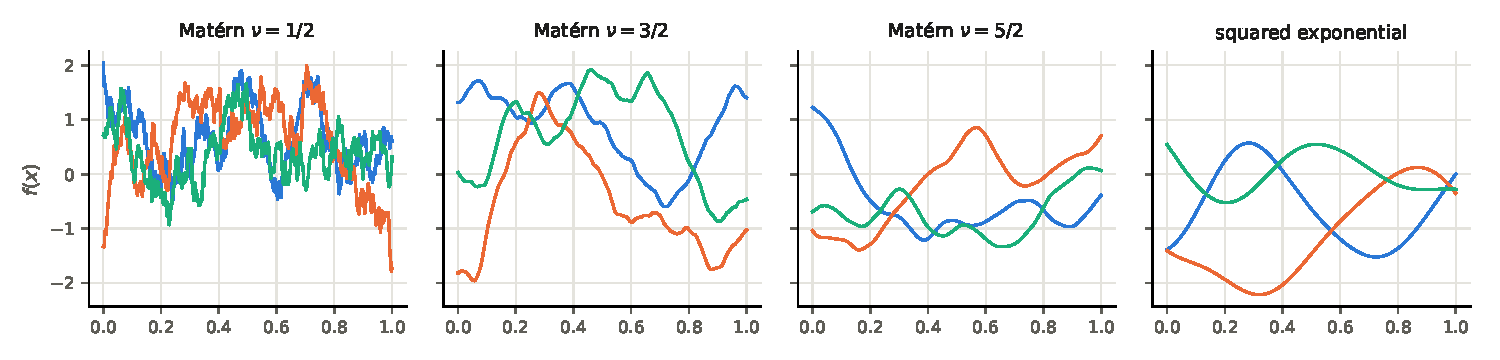
\includegraphics[width=\textwidth]{figures/ch02_prior_samples.pdf}
  \caption{Three random functions from each of four GP priors, all with length-scale $\ell = 0.2$. Same
  correlation distance, very different smoothness.}
  \label{fig:prior}
\end{figure}

\paragraph{The frequency view (Bochner's theorem).} A stationary kernel is valid exactly when it is the Fourier
transform of a nonnegative function $S(\omega)$, its \emph{spectral density}:
$k(\tau) = \int S(\omega)\, e^{i\omega\T\tau}\, d\omega$. The spectral density says how much variance sits at each
frequency. SE has a Gaussian spectrum, which decays faster than any power: high frequencies are essentially
forbidden, hence infinite smoothness. Mat\'ern-$\nu$ has $S(\omega) \propto (2\nu/\ell^2 + \norm{\omega}^2)^{-(\nu +
d/2)}$, a power-law tail: some high-frequency content survives, hence finite smoothness. Reading a kernel as a
filter on frequencies is the natural view for anyone who has done spectral analysis of flow fields.

\begin{connection}[Random Fourier features and the study's \texttt{gp\_draw} problems]
Bochner gives a cheap way to sample an approximate GP: draw frequencies $\omega_k$ from $S$, phases $b_k$ uniform,
and set $f(x) = \sqrt{2/D}\sum_{k=1}^D a_k \cos(\omega_k\T x + b_k)$ with $a_k \sim \N(0,1)$. This is a finite-feature
model of Chapter~\ref{ch:toolkit} whose kernel tends to $k$ as $D$ grows. The study's \texttt{gp\_draw} test
functions are built exactly this way (Student-$t$ frequencies, i.e.\ a Mat\'ern-5/2-like spectrum, $D = 256$).
\end{connection}

\section{Prediction: conditioning on the data}

Take a GP prior $f \sim \mathcal{GP}(0, k)$ (a nonzero mean is handled in Section~\ref{sec:kriging}) and noisy
observations $y_i = f(x_i) + \varepsilon_i$ with $\varepsilon_i \sim \N(0,\sigma_n^2)$ independent. At a new point
$x_*$, the pair $(f(x_*), y)$ is jointly Gaussian with
\begin{equation}
  \begin{pmatrix} f(x_*) \\ y \end{pmatrix} \sim
  \N\!\left(0,\; \begin{pmatrix} k(x_*,x_*) & k_*\T \\ k_* & K + \sigma_n^2 I \end{pmatrix}\right),
  \qquad K_{ij} = k(x_i,x_j),\; (k_*)_i = k(x_i, x_*).
\end{equation}
Conditioning (Result~\ref{res:condition}) gives the posterior at once:
\begin{equation}
  \boxed{\;
  \mu(x_*) = k_*\T (K + \sigma_n^2 I)^{-1} y, \qquad
  s^2(x_*) = k(x_*,x_*) - k_*\T (K + \sigma_n^2 I)^{-1} k_* .\;}
  \label{eq:gp_post}
\end{equation}

\paragraph{Reading the mean.} With $\alpha = (K + \sigma_n^2 I)^{-1} y$, the mean is
$\mu(x) = \sum_{i=1}^n \alpha_i\, k(x_i, x)$: a weighted sum of $n$ bumps, one centred on each data point, shaped
like the kernel. The surrogate is as smooth as the kernel, and its gradient is available analytically,
$\nabla\mu(x) = \sum_i \alpha_i \nabla_x k(x_i, x)$. This is why the study measured excellent gradients for the GP
family: the surrogate is a smooth sum of smooth bumps.

\paragraph{Reading the variance.} The variance starts at the prior $k(x_*,x_*)$ and subtracts what the data explain.
Near data it shrinks; far away it returns to the prior. Two consequences:
\begin{itemize}[nosep]
  \item With $\sigma_n = 0$ the mean interpolates ($\mu(x_i) = y_i$) and the variance is zero at the data. With
        noise, it smooths, and the variance at a data point is below $\sigma_n^2$ but not zero.
  \item \textbf{The variance does not depend on $y$.} It depends only on where you sampled. A sampling rule that
        adds the point of maximum variance therefore ignores what $f$ looked like there: it is a space-filling
        design in disguise. That is the mechanism behind the thesis-review finding (B-02) that the GP-variance scout
        performed about like a model-free maximin design. Only the hyper-parameters, refitted on the new data,
        carry information about $f$ into such a rule.
\end{itemize}

\paragraph{Computing it.} Never form an inverse. With one Cholesky factorisation:
\begin{enumerate}[nosep]
  \item $L = \operatorname{chol}(K + \sigma_n^2 I)$ \hfill $n^3/3$ operations, $n^2$ memory
  \item $\alpha = L\T \backslash (L \backslash y)$ \hfill two triangular solves, $2n^2$
  \item mean $\mu(x_*) = k_*\T\alpha$ \hfill $n$ per test point
  \item $v = L \backslash k_*$, variance $s^2(x_*) = k(x_*,x_*) - v\T v$ \hfill $n^2$ per test point
  \item $\log p(y) = -\tfrac12 y\T\alpha - \sum_i \log L_{ii} - \tfrac n2 \log 2\pi$ \hfill free (Section~\ref{sec:ml2})
\end{enumerate}
The $n^3$ step is why exact GPs stop at a few thousand points, and why the study caps the GP family at $n = 1000$.
Sparse GPs (later chapter) replace $K$ by a rank-$m$ approximation, reducing the cost to $n m^2$.

\section{Three names for one object}
\label{sec:kriging}

\paragraph{Kernel ridge regression.} Forget probability. Among all functions in a space $\mathcal{H}$, find
\begin{equation}
  \hat f = \argmin_{g \in \mathcal{H}} \sum_{i=1}^n \big(y_i - g(x_i)\big)^2 + \lambda \norm{g}_{\mathcal{H}}^2 .
  \label{eq:krr}
\end{equation}
For the right space (below) the answer is the GP mean \eqref{eq:gp_post} with $\lambda = \sigma_n^2$. This is the
infinite-dimensional version of Chapter~\ref{ch:toolkit}'s ``MAP is ridge''.

\paragraph{The space that makes it work.} The \emph{reproducing kernel Hilbert space} (RKHS) of $k$ is the space of
functions $g = \sum_j c_j\, k(z_j, \cdot)$ (and limits of such sums), with inner product
$\ip{k(x,\cdot)}{k(x',\cdot)}_{\mathcal{H}} = k(x,x')$. The defining \emph{reproducing property} is
\begin{equation}
  g(x) = \ip{g}{k(x,\cdot)}_{\mathcal{H}} \qquad\text{for every } g \in \mathcal{H}:
\end{equation}
evaluating a function at $x$ is taking its inner product with the kernel bump at $x$. The norm
$\norm{g}_{\mathcal{H}}$ measures roughness in the kernel's own terms; for Mat\'ern kernels it is equivalent to a
Sobolev norm (an integral of squared derivatives up to order $\nu + d/2$), the same kind of ``energy'' as in a
variational formulation of a PDE.

\begin{result}[Representer theorem]
The minimiser of \eqref{eq:krr} has the form $\hat f(x) = \sum_{i=1}^n \alpha_i\, k(x_i, x)$: only the bumps at the
data are ever needed, even though $\mathcal{H}$ is infinite-dimensional.
\end{result}
\begin{intuition}
Projection again. Split any candidate $g = g_\parallel + g_\perp$, with $g_\parallel$ in the span of the data bumps
$k(x_i,\cdot)$ and $g_\perp$ orthogonal to all of them. By the reproducing property
$g_\perp(x_i) = \ip{g_\perp}{k(x_i,\cdot)} = 0$, so $g_\perp$ is invisible at the data: the fit term is unchanged.
But $\norm{g}^2 = \norm{g_\parallel}^2 + \norm{g_\perp}^2$ (Pythagoras), so $g_\perp$ only adds penalty. The best
choice is $g_\perp = 0$.
\end{intuition}

\paragraph{Radial basis function interpolation.} RBF interpolation, from approximation theory and engineering,
writes $s(x) = \sum_i c_i\, \varphi(\norm{x - x_i})$ and solves for $c$ so that $s(x_i) = y_i$. With $\varphi$ a
PD kernel this is the noise-free GP mean ($\sigma_n = 0$). Some popular radial functions (multiquadric, thin-plate
spline $r^2\log r$) are only \emph{conditionally} PD, which is repaired by adding a low-degree polynomial and
orthogonality conditions; the thin-plate spline minimises a bending energy, its RKHS-type seminorm.

\paragraph{Kriging.} Geostatistics (Krige, Matheron) derived the same predictor as the best linear unbiased predictor
of a spatial field. \emph{Simple kriging} assumes a known mean (our zero-mean GP). \emph{Ordinary kriging} assumes an
unknown constant mean $\beta$ and estimates it by generalised least squares, $\hat\beta = (\mathbf{1}\T A^{-1}y) /
(\mathbf{1}\T A^{-1}\mathbf{1})$ with $A = K + \sigma_n^2 I$, then kriges the residual. \emph{Universal kriging}
replaces the constant by a regression on basis functions. ``Kriging'' in engineering software (DACE, SMT) is a GP
with one of these means.

\begin{intuition}
Kriging, GP regression, kernel ridge regression and RBF interpolation produce the same prediction for the same
kernel and noise level. They differ in what else they give you and in how they choose hyper-parameters: the GP gives
a variance and a likelihood for choosing $\ell$, KRR usually picks $\lambda$ and $\ell$ by cross-validation, RBF
practice often fixes them by rule. In the study's results this is visible: \texttt{krr}, the RBFs and the GP family
are neighbours in accuracy, and their differences come mostly from hyper-parameter choice.
\end{intuition}

\section{What the error bar means}

\begin{result}[The GP variance is a worst-case error bound]
\label{res:power}
For noise-free data, the mean $\mu$ of \eqref{eq:gp_post} satisfies, for every $f$ in the RKHS,
\begin{equation}
  |f(x) - \mu(x)| \;\le\; s_0(x)\, \norm{f}_{\mathcal{H}} ,
\end{equation}
where $s_0^2(x)$ is the noise-free posterior variance (called the \emph{power function} in approximation theory).
\end{result}
\begin{intuition}
The interpolant is linear in the data: $\mu(x) = \sum_i c_i(x) f(x_i)$ for weights $c(x) = K^{-1}k_*$. By the
reproducing property,
$f(x) - \mu(x) = \ip{f}{k(x,\cdot) - \sum_i c_i(x) k(x_i,\cdot)}_{\mathcal{H}}$, and Cauchy--Schwarz bounds this by
$\norm{f}_{\mathcal{H}}$ times the norm of the second factor. Expanding that norm with $\ip{k(a,\cdot)}{k(b,\cdot)} =
k(a,b)$ gives exactly $k(x,x) - k_*\T K^{-1} k_*$. So the GP's error bar is not only a Bayesian belief; it is the
largest possible error over all functions of a given RKHS norm, i.e.\ of a given roughness.
\end{intuition}

\paragraph{Rates.} For Mat\'ern-$\nu$ kernels the power function shrinks like $h^{\nu}$, where the \emph{fill distance}
$h$ is the radius of the largest empty ball among the samples. A good space-filling design has $h \approx n^{-1/d}$,
so the error falls like $n^{-\nu/d}$: Chapter~\ref{ch:toolkit}'s rate with $s = \nu$, now as a theorem. Two caveats
the study sees in practice: the bound needs $f$ to be in the RKHS (a discontinuous $f$ is not, and the GP converges
slowly near jumps), and it needs the right $\ell$, which brings us to the hard part.

\section{Choosing hyper-parameters: the marginal likelihood}
\label{sec:ml2}

The kernel has hyper-parameters $\theta = (\sigma_f, \ell_1,\dots,\ell_d, \sigma_n)$. Integrating $f$ out
(a linear-Gaussian computation) gives the probability of the data under $\theta$, the \emph{marginal likelihood} or
\emph{evidence}: $y \mid \theta \sim \N(0, A_\theta)$ with $A_\theta = K_\theta + \sigma_n^2 I$, so
\begin{equation}
  \log p(y\mid\theta) =
  \underbrace{-\tfrac12\, y\T A_\theta^{-1} y}_{\text{data fit}}
  \;\underbrace{-\;\tfrac12 \log\det A_\theta}_{\text{complexity penalty}}
  \;-\; \tfrac n2 \log 2\pi .
  \label{eq:lml}
\end{equation}
Maximising it over $\theta$ is \emph{type-II maximum likelihood} (ML-II), the default in every GP package.

\begin{intuition}[Automatic Occam's razor]
The first term rewards explaining the data. The second term is a penalty: $\det A_\theta$ measures the volume of data
sets the model considers plausible, so a very flexible model (short $\ell$, large $\sigma_f$) spreads its probability
over many possible data sets and assigns less to the one observed. A model that is too rigid cannot explain the
data; one that is too flexible could explain anything and is therefore unconvincing about this data set. The evidence
peaks in between. Its gradient is available in closed form,
$\partial_\theta \log p = \tfrac12 \alpha\T(\partial_\theta A)\alpha - \tfrac12 \tr(A^{-1}\partial_\theta A)$, and
L-BFGS does the rest.
\end{intuition}

\subsection{Where ML-II goes wrong}

The evidence is not concave in $\theta$, and with few points it can prefer nonsense. Both failures appeared in the
study, so here they are explicitly.

\paragraph{Several local optima.} Figure~\ref{fig:lml} shows the evidence (with $\sigma_f$ optimised out) for 40 noisy
samples of $\sin(2\pi x) + 0.3\sin(20\pi x)$. There are two peaks. One, at $\ell = 0.051$ and noise/signal ratio
$0.003$ (log evidence $-9.2$), fits both components. The other, at $\ell = 0.22$ and ratio $0.087$ ($-17.5$),
explains the slow component and calls the fast one noise. Both are reasonable stories; a gradient optimizer started
near the second never finds the first. This is the ``signal fitted as noise'' failure of bug N-14.

\begin{figure}[t]
  \centering
  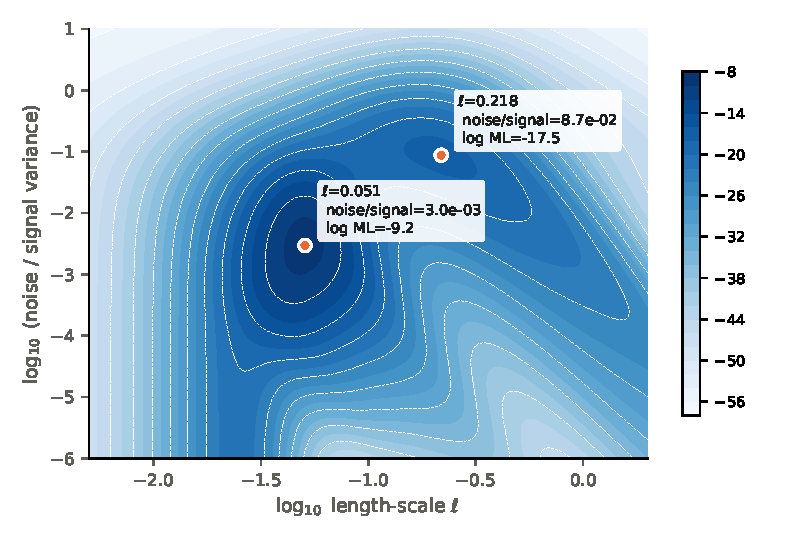
\includegraphics[width=0.66\textwidth]{figures/ch02_lml_landscape.pdf}
  \caption{Log marginal likelihood over length-scale and noise ratio for a slow-plus-fast signal. Two local maxima
  (orange): ``fit everything'' and ``fast part is noise''. Which one an optimizer reaches depends on where it
  starts.}
  \label{fig:lml}
\end{figure}

\paragraph{Too few points: the length-scale collapses.} Figure~\ref{fig:post} fits a GP to six points of the
Forrester function. With $\ell$ fixed at a sensible $0.15$, the fit is good (NRMSE $0.125$). Letting ML-II choose,
with ten restarts, drives $\ell$ to its lower bound $0.01$: the posterior mean becomes a row of spikes at the data
and the prior mean everywhere else (NRMSE $0.94$). And the evidence genuinely prefers it: $-8.51$ against $-9.24$.
With six points, ``independent values at each sample'' is a perfectly good explanation of six numbers, and
it costs less complexity than a smooth function that must bend through all of them. The data cannot rule it out.

\begin{figure}[t]
  \centering
  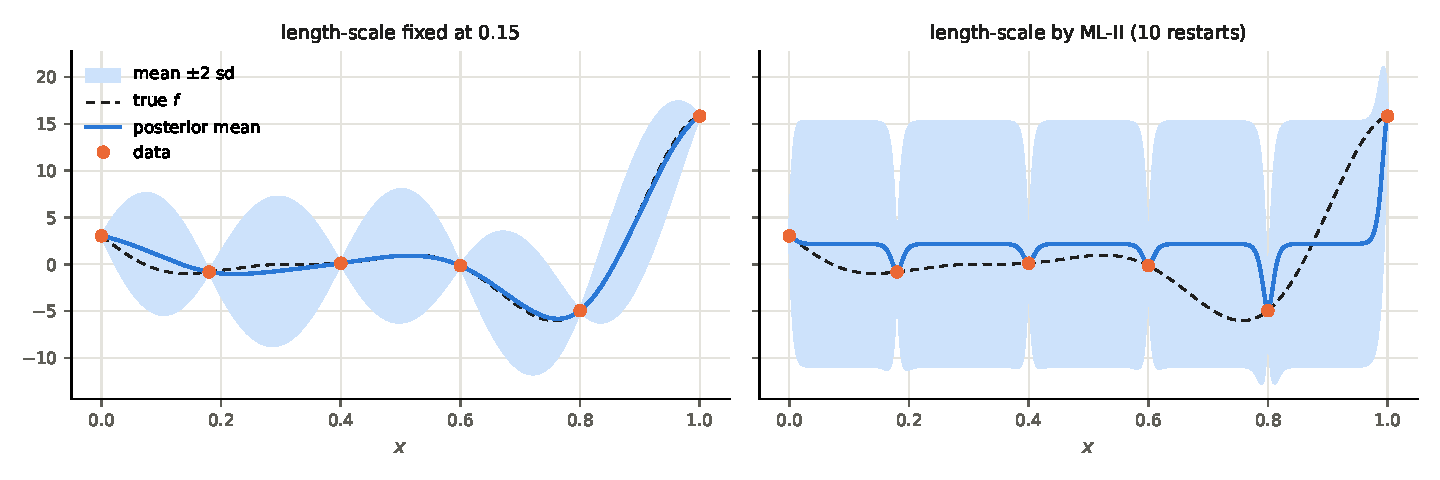
\includegraphics[width=\textwidth]{figures/ch02_posterior.pdf}
  \caption{GP fits to six samples of the Forrester function. Left: length-scale fixed at 0.15. Right: length-scale
  chosen by ML-II, which collapses to its bound (0.01) and returns the prior between samples. Note how the variance
  band (shaded) reflects only the spacing of the samples, not the values.}
  \label{fig:post}
\end{figure}

\paragraph{Ill-conditioning.} For 50 evenly spaced points on $[0,1]$, the condition number of $K$:
\begin{center}
\begin{tabular}{lrrr}
\toprule
length-scale $\ell$ & SE & Mat\'ern 5/2 & Mat\'ern 1/2 \\
\midrule
0.02 & $5.6\times10^{1}$ & $1.2\times10^{1}$ & 4.5 \\
0.05 & $1.1\times10^{12}$ & $1.0\times10^{3}$ & 24 \\
0.1  & $1.6\times10^{18}$ & $5.4\times10^{4}$ & 91 \\
0.2  & $1.3\times10^{19}$ & $3.0\times10^{6}$ & 320 \\
0.5  & $1.4\times10^{19}$ & $5.1\times10^{8}$ & $1.4\times10^{3}$ \\
\bottomrule
\end{tabular}
\end{center}
When samples are close relative to $\ell$, neighbouring columns of $K$ are nearly identical (the monomial problem of
Chapter~\ref{ch:toolkit} again). SE is the worst because its spectrum dies fastest: its eigenvalues $\lambda_j$ decay
super-exponentially, so $K$ is numerically singular beyond $\ell \approx 0.05$ here. Adding a \emph{nugget} (a small
$\sigma_n^2$, or ``jitter'') shifts every eigenvalue up and is exactly Chapter~\ref{ch:toolkit}'s ridge filter. It is
one reason the study prefers Mat\'ern 5/2 to SE, and why every GP in the study has a nugget floor.

\paragraph{What the study found, and the remedies.} In E3 between 2 and 9\% of GP-family fits (1 restart) were more
than twice as bad as a kernel ridge regression on the same data, the signature of a bad optimum, and five restarts
fixed most of them. Standard remedies, in increasing cost: several restarts; sensible bounds (a length-scale floor
near the smallest sample spacing rules out the collapse above); a prior on $\theta$ and maximising the posterior
instead of the likelihood (``MAP-II''); choosing $\theta$ by cross-validation; and, most robust, averaging over
$\theta$ with Markov-chain Monte Carlo instead of choosing one value. Kernel Flows, used by one of the study's
learners, is a cross-validation-like criterion built for exactly this problem.

\section{When a GP is the wrong model}

\begin{center}
\small
\begin{tabular}{p{4.1cm}p{5.3cm}p{4.2cm}}
\toprule
Property of $f$ & Why a stationary GP struggles & Variant (later chapters) \\
\midrule
Jumps, kinks & not in the RKHS; one global $\ell$ must be short everywhere, so oscillation (Gibbs-like) near the jump &
treed GP, local GP, partitioned models \\
Nonstationary (rough here, smooth there) & one length-scale for the whole domain & warped GP, deep GP, Kernel
Flows \\
Noise that varies or has outliers & Gaussian likelihood, constant $\sigma_n$ & heteroscedastic GP, Student-$t$
likelihood \\
High dimension & distances concentrate; $d$ length-scales to fit & ARD, active-subspace GP, KPLS \\
Large $n$ & $n^3$ cost, $n^2$ memory & sparse GP, local GP \\
\bottomrule
\end{tabular}
\end{center}

The study's E3 results line up with this table: GP variants win smooth, ridge, multiscale and engineering problems
(where $f$ is in the RKHS of a Mat\'ern kernel with sensible length-scales), and lose discontinuities and steep drops
to trees.

\section*{Notes}
\begin{itemize}[leftmargin=*,nosep]
  \item Derivatives of a GP are again a GP (differentiation is linear), with covariance $\partial_x\partial_{x'}k$.
        Gradient observations can therefore be conditioned on exactly like values: gradient-enhanced kriging, the
        subject of the planned gradient study (E13).
  \item Multi-output and multi-fidelity GPs (co-kriging) use a kernel on (input, output index); a later chapter.
\end{itemize}

\section*{Summary of the formulas to keep}
\begin{itemize}[nosep]
  \item GP posterior: $\mu = k_*\T(K + \sigma_n^2 I)^{-1}y$, $s^2 = k_{**} - k_*\T(K + \sigma_n^2 I)^{-1}k_*$: Gaussian
        conditioning, computed with one Cholesky factorisation.
  \item The mean is $\sum_i \alpha_i k(x_i, \cdot)$ (representer theorem); the variance ignores $y$.
  \item Kriging $=$ GP mean $=$ kernel ridge regression ($\lambda = \sigma_n^2$) $=$ RBF interpolation
        ($\sigma_n = 0$).
  \item Mat\'ern $\nu$ = smoothness $s$; error $\le s_0(x)\norm{f}_{\mathcal{H}}$ and $\approx n^{-\nu/d}$.
  \item Evidence = data fit $-$ complexity; non-concave, can collapse with few points; restarts, bounds, priors,
        nugget.
\end{itemize}
